\documentclass[]{article}
\usepackage{lmodern}
\usepackage{amssymb,amsmath}
\usepackage{ifxetex,ifluatex}
\usepackage{fixltx2e} % provides \textsubscript
\ifnum 0\ifxetex 1\fi\ifluatex 1\fi=0 % if pdftex
  \usepackage[T1]{fontenc}
  \usepackage[utf8]{inputenc}
\else % if luatex or xelatex
  \ifxetex
    \usepackage{mathspec}
  \else
    \usepackage{fontspec}
  \fi
  \defaultfontfeatures{Ligatures=TeX,Scale=MatchLowercase}
  \newcommand{\euro}{€}
\fi
% use upquote if available, for straight quotes in verbatim environments
\IfFileExists{upquote.sty}{\usepackage{upquote}}{}
% use microtype if available
\IfFileExists{microtype.sty}{%
\usepackage{microtype}
\UseMicrotypeSet[protrusion]{basicmath} % disable protrusion for tt fonts
}{}
\usepackage[margin=1in]{geometry}
\usepackage{hyperref}
\PassOptionsToPackage{usenames,dvipsnames}{color} % color is loaded by hyperref
\hypersetup{unicode=true,
            pdftitle={REF IR/Political Science Prediction Models (version 0.3)},
            pdfauthor={Christopher Gandrud},
            pdfborder={0 0 0},
            breaklinks=true}
\urlstyle{same}  % don't use monospace font for urls
\usepackage{longtable,booktabs}
\usepackage{graphicx,grffile}
\makeatletter
\def\maxwidth{\ifdim\Gin@nat@width>\linewidth\linewidth\else\Gin@nat@width\fi}
\def\maxheight{\ifdim\Gin@nat@height>\textheight\textheight\else\Gin@nat@height\fi}
\makeatother
% Scale images if necessary, so that they will not overflow the page
% margins by default, and it is still possible to overwrite the defaults
% using explicit options in \includegraphics[width, height, ...]{}
\setkeys{Gin}{width=\maxwidth,height=\maxheight,keepaspectratio}
\setlength{\parindent}{0pt}
\setlength{\parskip}{6pt plus 2pt minus 1pt}
\setlength{\emergencystretch}{3em}  % prevent overfull lines
\providecommand{\tightlist}{%
  \setlength{\itemsep}{0pt}\setlength{\parskip}{0pt}}
\setcounter{secnumdepth}{0}

%%% Use protect on footnotes to avoid problems with footnotes in titles
\let\rmarkdownfootnote\footnote%
\def\footnote{\protect\rmarkdownfootnote}

%%% Change title format to be more compact
\usepackage{titling}

% Create subtitle command for use in maketitle
\newcommand{\subtitle}[1]{
  \posttitle{
    \begin{center}\large#1\end{center}
    }
}

\setlength{\droptitle}{-2em}
  \title{REF IR/Political Science Prediction Models (version 0.3)}
  \pretitle{\vspace{\droptitle}\centering\huge}
  \posttitle{\par}
  \author{Christopher Gandrud}
  \preauthor{\centering\large\emph}
  \postauthor{\par}
  \predate{\centering\large\emph}
  \postdate{\par}
  \date{25 February 2016}



% Redefines (sub)paragraphs to behave more like sections
\ifx\paragraph\undefined\else
\let\oldparagraph\paragraph
\renewcommand{\paragraph}[1]{\oldparagraph{#1}\mbox{}}
\fi
\ifx\subparagraph\undefined\else
\let\oldsubparagraph\subparagraph
\renewcommand{\subparagraph}[1]{\oldsubparagraph{#1}\mbox{}}
\fi

\begin{document}
\maketitle

I conducted a simple Random Forest Regression to examine how
IR/Political Science REF 2014 Output GPAs could be predicted using:

\begin{itemize}
\item
  \textbf{Mean Journal Impact Factor} for all of the journal article
  submissions that each university made. Note: if a journal was not
  assigned an impact factor\footnote{E.g. new journals and journals not
    included in the impact factor list used. Note that we attempted to
    match all of the submitted articles' journal names with those on the
    impact factor list. However, due to spelling variations in the two
    sets of journal names, some matches may not have been made.} it is
  effectively given an impact factor of 0.
\item
  \textbf{Percent of journal article} submissions from journals in the
  \textbf{top 20} IR or Political Science categories assembled by Google
  Scholar.
\item
  \textbf{Percent of non-edited books} submitted that were published by
  a \textbf{top university press} (see table in the Appendix for the
  complete list).
\end{itemize}

All of these metrics are highly correlated with REF Output GPAs. Mean
impact factor has a correlation coefficient of 0.68 with REF Output
GPAs. The REF GPA correlation with the Google Scholar metric is 0.76 and
0.7 with the percentage of books submitted that were published by a top
university press. The following figure further illustrates these close
relationships and City University's placement within them.

It is important to note that neither of these metrics contain
information on other materials including edited volues which are also
submitted to the REF.

\begin{figure}[htbp]
\centering
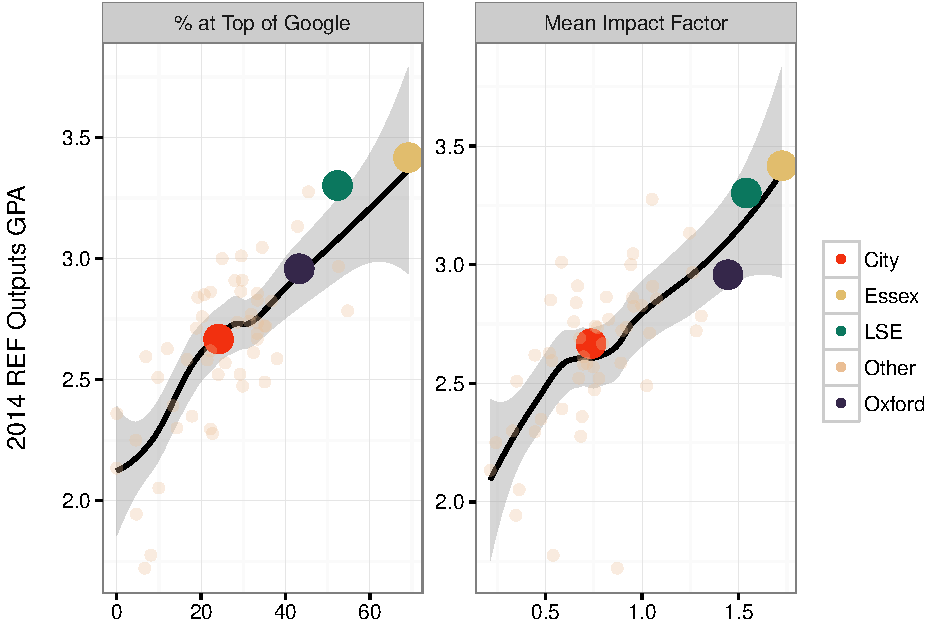
\includegraphics{README_files/figure-latex/descript-1.pdf}
\caption{Comparing Universities' REF 2014 Output GPA to Journal Research
Output Metrics}
\end{figure}

\section{More Complex Model: Google Scholar + Impact Factor +
Books}\label{more-complex-model-google-scholar-impact-factor-books}

To examine how well these metrics predict REF Output GPAs I first ran
the random forest regression model on a random sample of 70\% of the 56
universities (i.e.~38) that made REF submissions for IR/Political
Science. I then used the estimates from the model to predict the REF
Output scores of the remaining 30\% (i.e.~17 universities). The
following figure compares the actual REF GPA scores to the predictions.
Note: if the model perfectly predicted the GPA score then each dot would
lie one the 45 degree line. The mean absolute prediction error when
using the two journal metrics was 0.1. In other words, on average the
model incorrectly predicted the REF GPA score by 0.1 GPA points or 2.5\%
of the GPA scale.

\begin{figure}[htbp]
\centering
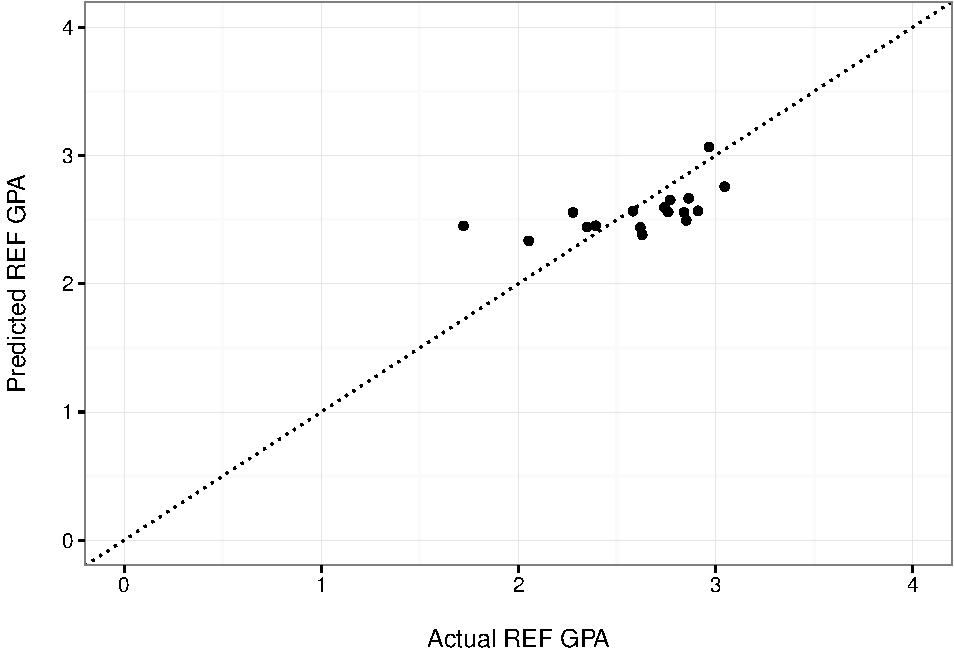
\includegraphics{README_files/figure-latex/unnamed-chunk-1-1.pdf}
\caption{Actual vs.~Predicted 2014 REF Output GPAs Using All Output
Metrics for a Test Set of 17 Randomly Selected Universities}
\end{figure}

\section{Simpler model: Google Scholar
Only}\label{simpler-model-google-scholar-only}

The percentage of journal submissions in the top Google Scholar lists is
more strongly correlated with REF GPA scores than impact factors. Would
a simpler model using just the Google Scholar metric perform just as
well as the more complex two metric model? The following figures shows
actual vs.~predicted GPA scores for this model. The mean absolute
prediction error when using only the Google Scholar metric was 0.2. In
other words, on average the model incorrectly predicted the REF GPA
score by 0.2 GPA points or 5\% of the GPA scale. The Google Scholar Only
model slightly outperforms the more complex model that also included
information on impact factors.

\begin{figure}[htbp]
\centering
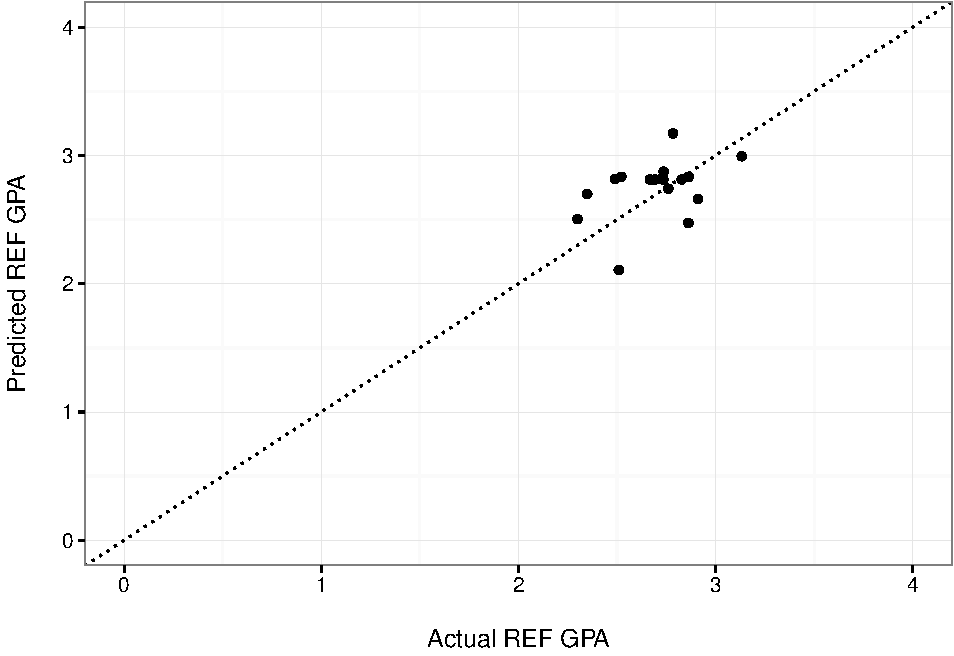
\includegraphics{README_files/figure-latex/unnamed-chunk-3-1.pdf}
\caption{Actual vs.~Predicted 2014 REF Output GPAs Using Google Scholar
Metric for a Test Set of 17 Randomly Selected Universities}
\end{figure}

\section{Simple, But a Little More Complex: Google
Plus}\label{simple-but-a-little-more-complex-google-plus}

The Google Top 20 IR and Political Science lists are notably lacking
important political economy journals, including \emph{Review of
International Political Economy} and \emph{New Political Economy}. Does
adding these journals to a ``Google Scholar Plus'' variable improve
prediction performance? The following figure shows the predicted
vs.~actual REF GPAs for our test sample using the Google Scholar Plus
variable. The mean absolute prediction error when using only the Google
Scholar Plus metric was 0.174. In other words, on average the model
incorrectly predicted the REF GPA score by 0.174 GPA points or 4.4\% of
the GPA scale. The Google Scholar Plus model slightly outperforms both
the Two Metric model and the Google Scholar Only model.

\begin{figure}[htbp]
\centering
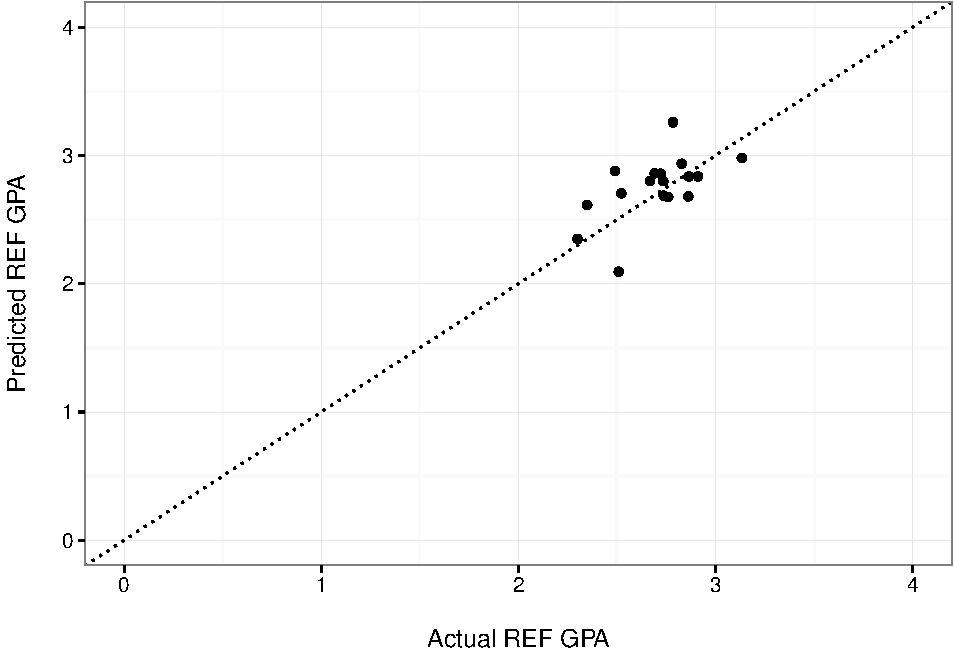
\includegraphics{README_files/figure-latex/unnamed-chunk-4-1.pdf}
\caption{Actual vs.~Predicted 2014 REF Output GPAs Using Google Scholar
Plus Metric for a Test Set of 17 Randomly Selected Universities}
\end{figure}

\section{Conclusion}\label{conclusion}

For the International Relations/Political Science 2014 REF we can create
highly accurate predictions of Output GPA using only universities'
percentage of journal submissions that were from the Google Scholar IR
and Political Science top 20 lists. Using subject specific knowledge to
select two additional journals that are prominent in international
political economy allows us to make even better predictions. It may be
possible to make even better predictions by including information on
high impact book publishers.

\section{Appendix: Top 20 (IR + PS) Google Scholar Journals (February
2016)}\label{appendix-top-20-ir-ps-google-scholar-journals-february-2016}

For reference, the following is a list of the top 20 journals in the
Google Scholar IR and Political Science categories. We also include the
most recent Thomson-Reuters Impact factor to enable comparison between
the two metrics. Note that the table does not include 40 journals
because some journals (\emph{World Politics} and \emph{Journal of
Democracy} show up on both the IR and Political Science lists).

\begin{longtable}[c]{@{}lr@{}}
\toprule
Journal & TR Impact Factor\tabularnewline
\midrule
\endhead
political analysis & 4.655\tabularnewline
american political science review & 3.688\tabularnewline
journal of peace research & 3.387\tabularnewline
american journal of political science & 3.269\tabularnewline
annual review of political science & 3.140\tabularnewline
international organization & 3.019\tabularnewline
european journal of political research & 2.508\tabularnewline
world politics & 2.450\tabularnewline
journal of politics & 2.255\tabularnewline
governance & 2.237\tabularnewline
perspectives on politics & 2.132\tabularnewline
comparative political studies & 2.028\tabularnewline
foreign affairs & 2.009\tabularnewline
british journal of political science & 1.987\tabularnewline
european journal of international relations & 1.972\tabularnewline
jcms & 1.855\tabularnewline
party politics & 1.830\tabularnewline
journal of european public policy & 1.817\tabularnewline
international studies quarterly & 1.705\tabularnewline
political behavior & 1.691\tabularnewline
journal of conflict resolution & 1.609\tabularnewline
west european politics & 1.576\tabularnewline
security dialogue & 1.356\tabularnewline
international affairs & 1.246\tabularnewline
electoral studies & 1.182\tabularnewline
journal of democracy & 1.180\tabularnewline
political research quarterly & 1.149\tabularnewline
review of international studies & 1.087\tabularnewline
global governance & 1.016\tabularnewline
third world quarterly & 0.981\tabularnewline
political studies & 0.939\tabularnewline
international studies review & 0.878\tabularnewline
millennium & 0.841\tabularnewline
washington quarterly & 0.788\tabularnewline
journal of european integration & 0.656\tabularnewline
international studies perspectives & 0.652\tabularnewline
pacific review & 0.527\tabularnewline
ethics \& international affairs & 0.453\tabularnewline
\bottomrule
\end{longtable}

\end{document}
